% ============================================================
% Part 2：原文第 17-32 页
% （3.2.1 数学记法与内存顺序 …… 4.3 AdamW，Problem (adamw_accounting) 开头）
% ============================================================

……在使用 einsum 记法的代码中，输入和输出张量的相关形状会清楚得多。对于其余的张量，你可以考虑使用 Tensor 类型标注，例如使用 jaxtyping 库（它并非 JAX 专属）。

关于使用 einsum 记法对性能的影响，我们会在作业 2 中进一步讨论；但现在你只需要知道：einsum 几乎总是比其他写法更好！

\subsubsection{数学记法与内存顺序（Mathematical Notation and Memory Ordering）}

许多机器学习论文在记法中使用行向量，这种表示与 NumPy 和 PyTorch 默认采用的行主序（row-major）内存布局十分契合。采用行向量时，线性变换写作
\begin{equation}
y = xW^{\top},
\tag{1}
\end{equation}
其中按行主序存储的 $W \in \mathbb{R}^{d_{\mathrm{out}} \times d_{\mathrm{in}}}$，行向量 $x \in \mathbb{R}^{1 \times d_{\mathrm{in}}}$。注意，这种写法让我们可以通过增加 $x$ 的最外层维度来对输入做批处理（batching），也就是说，可以把向量输入 $x$ 替换为矩阵输入 $X \in \mathbb{R}^{\mathrm{batch} \times d_{\mathrm{in}}}$。

在线性代数中，更常见的是使用列向量，此时线性变换写作
\begin{equation}
y = Wx,
\tag{2}
\end{equation}
其中 $W \in \mathbb{R}^{d_{\mathrm{out}} \times d_{\mathrm{in}}}$ 按行主序存储，$x \in \mathbb{R}^{d_{\mathrm{in}}}$ 是列向量。在这种设定下若要对输入做批处理，批次维度必须放在 $x$ 的最后，因此 $x$ 需要替换为矩阵 $\tilde{X} \in \mathbb{R}^{d_{\mathrm{in}} \times \mathrm{batch}}$。

\textbf{在本作业的数学记法中，我们主要使用列向量}，因为数学文献通常遵循这一记法。请记住：如果你想使用朴素的矩阵乘法记号，由于 PyTorch 采用行主序内存布局，就必须像式~(1) 的行向量约定那样，在应用矩阵时多做一次转置。如果你的线性代数运算都使用 \tm{einsum} 来写，那么只要轴标签标注正确，这完全不成问题。顺带一提，值得注意的是，其他语言或线性代数软件包（如 Matlab、Julia 和 Fortran）都使用列主序（column-major）内存布局，即批次维度放在最后；而 Python 及其相关软件包采用的是 C 语言标准的行主序布局。

\subsection{基础构建模块：Linear 与 Embedding 模块}

\subsubsection{参数初始化（Parameter Initialization）}

要有效地训练神经网络，通常需要仔细地初始化模型参数——糟糕的初始化会导致梯度消失或梯度爆炸等不良行为。Pre-norm Transformer 对初始化出奇地鲁棒，但初始化仍然会显著影响训练速度和收敛性。由于本作业已经很长，我们把细节留到作业 3 再讲，这里直接给出一些在大多数情况下都应该能正常工作的近似初始化方法。目前请使用：

\begin{itemize}
  \item Linear 权重：$\mathcal{N}\bigl(\mu = 0,\ \sigma^2 = \tfrac{2}{d_{\mathrm{in}} + d_{\mathrm{out}}}\bigr)$，截断（truncated）于 $[-3\sigma, 3\sigma]$。
  \item Embedding：$\mathcal{N}(\mu = 0,\ \sigma^2 = 1)$，截断于 $[-3, 3]$。
  \item RMSNorm：$1$。
\end{itemize}

你应该使用 \tm{torch.nn.init.trunc\_normal\_} 来初始化这些截断正态权重。

\subsubsection{Linear 模块（Linear Module）}

线性层是 Transformer 乃至一般神经网络的基础构建模块。首先，你要实现自己的 \tm{Linear} 类，它继承自 \tm{torch.nn.Module} 并执行线性变换
\begin{equation}
y = Wx.
\tag{3}
\end{equation}
注意：与大多数现代大语言模型一致，我们不包含偏置（bias）项。

\subsubsection*{问题（linear）：实现 Linear 模块（1 分）}

\textbf{交付要求：}实现一个继承自 \tm{torch.nn.Module} 并执行线性变换的 \tm{Linear} 类。你的实现应当遵循 PyTorch 内置 \tm{nn.Linear} 模块的接口，但不带 \tm{bias} 参数（argument）或参数（parameter）。我们推荐如下接口：

\tm{def \_\_init\_\_(self, in\_features, out\_features, device=None, dtype=None)}\quad 构造线性变换模块。该函数应接受以下参数：
\begin{itemize}
  \item \tm{in\_features: int}：输入的最终维度。
  \item \tm{out\_features: int}：输出的最终维度。
  \item \tm{device: torch.device | None = None}：参数存储所在的设备。
  \item \tm{dtype: torch.dtype | None = None}：参数的数据类型。
\end{itemize}

\tm{def forward(self, x: torch.Tensor) -> torch.Tensor}\quad 对输入施加线性变换。

请务必做到：
\begin{itemize}
  \item 继承 \tm{nn.Module}；
  \item 调用父类构造函数；
  \item 把参数构造并存储为 $W$（而不是 $W^{\top}$），并放入 \tm{nn.Parameter}；
  \item 当然，不要使用 \tm{nn.Linear} 或 \tm{nn.functional.linear}。
\end{itemize}

初始化时，请使用上面的设置，并用 \tm{torch.nn.init.trunc\_normal\_} 初始化权重。

要测试你的 \tm{Linear} 模块，请在 \tm{[adapters.run\_linear]} 处实现测试适配器（adapter）。适配器应把给定的权重加载进你的 \tm{Linear} 模块，为此你可以使用 \tm{Module.load\_state\_dict}。然后运行 \tm{uv run pytest -k test\_linear}。

\subsubsection{Embedding 模块（Embedding Module）}

如上所述，Transformer 的第一层是嵌入层（embedding layer），它把整数 token ID 映射到维度为 \tm{d\_model} 的向量空间。我们将实现一个继承自 \tm{torch.nn.Module} 的自定义 \tm{Embedding} 类（因此不应使用 \tm{nn.Embedding}）。\tm{forward} 方法应通过索引形状为 \tm{(vocab\_size, d\_model)} 的嵌入矩阵，为每个 token ID 选出对应的嵌入向量，其中 token ID 是形状为 \tm{(batch\_size, sequence\_length)} 的 \tm{torch.LongTensor}。

\subsubsection*{问题（embedding）：实现 embedding 模块（1 分）}

\textbf{交付要求：}实现继承自 \tm{torch.nn.Module} 并执行嵌入查表（embedding lookup）的 \tm{Embedding} 类。你的实现应当遵循 PyTorch 内置 \tm{nn.Embedding} 模块的接口。我们推荐如下接口：

\tm{def \_\_init\_\_(self, num\_embeddings, embedding\_dim, device=None, dtype=None)}\quad 构造嵌入模块。该函数应接受以下参数：
\begin{itemize}
  \item \tm{num\_embeddings: int}：词表大小。
  \item \tm{embedding\_dim: int}：嵌入向量的维度，即 $d_{\mathrm{model}}$。
  \item \tm{device: torch.device | None = None}：参数存储所在的设备。
  \item \tm{dtype: torch.dtype | None = None}：参数的数据类型。
\end{itemize}

\tm{def forward(self, token\_ids: torch.Tensor) -> torch.Tensor}\quad 为给定的 token ID 查出嵌入向量。

请务必做到：
\begin{itemize}
  \item 继承 \tm{nn.Module}；
  \item 调用父类构造函数；
  \item 把嵌入矩阵初始化为 \tm{nn.Parameter}；
  \item 存储嵌入矩阵时，令 \tm{d\_model} 为最终维度；
  \item 当然，不要使用 \tm{nn.Embedding} 或 \tm{nn.functional.embedding}。
\end{itemize}

同样，请使用上面的设置进行初始化，并用 \tm{torch.nn.init.trunc\_normal\_} 初始化权重。

要测试你的实现，请在 \tm{[adapters.run\_embedding]} 处实现测试适配器，然后运行 \tm{uv run pytest -k test\_embedding}。

\subsection{Pre-Norm Transformer 块}

每个 Transformer 块都有两个子层（sub-layer）：多头自注意力机制和一个逐位置前馈网络（position-wise feed-forward network）（见 A.~Vaswani et al., 2017，第 3.1 节）。

在最初的 Transformer 论文中，模型在两个子层各自外围使用残差连接（residual connection），随后做层归一化（layer normalization）。这种架构通常被称为 ``post-norm'' Transformer，因为层归一化作用在子层的输出上。然而，多项工作发现，把层归一化从每个子层的输出移到每个子层的输入处（并在最后一个 Transformer 块之后额外加一层归一化）可以提升 Transformer 的训练稳定性（T.~Q.~Nguyen et al., 2019；R.~Xiong et al., 2020）——这种 ``pre-norm'' Transformer 块的可视化表示见图~2。随后，Transformer 块每个子层的输出经由残差连接加回到子层的输入上（A.~Vaswani et al.~[8]，第 5.4 节）。对 pre-norm 的一个直观理解是：存在一条从输入嵌入直通 Transformer 最终输出、不经过任何归一化的干净的``残差流（residual stream）''，据称这能改善梯度的流动。这种 pre-norm Transformer 如今已是语言模型的标准配置（例如 GPT-3、LLaMA、PaLM 等），因此我们将实现这一变体。下面我们会逐一介绍 pre-norm Transformer 块的各个组件，并依次实现它们。

\subsubsection{均方根层归一化（Root Mean Square Layer Normalization）}

最初的 Transformer 实现（A.~Vaswani et al.~[8]）使用层归一化（J.~L.~Ba et al., 2016）来归一化激活值。参照 H.~Touvron et al.~[12]，我们将使用均方根层归一化（root mean square layer normalization，RMSNorm；B.~Zhang et al.~[13]，式 4）来做层归一化。给定激活值向量 $a \in \mathbb{R}^{d_{\mathrm{model}}}$，RMSNorm 会按下式重新缩放每个激活值 $a_i$：
\begin{equation}
\operatorname{RMSNorm}(a_i) = \frac{a_i}{\operatorname{RMS}(a)}\, g_i,
\tag{4}
\end{equation}
其中 $\operatorname{RMS}(a) = \sqrt{\tfrac{1}{d_{\mathrm{model}}} \sum_{i=1}^{d_{\mathrm{model}}} a_i^2 + \varepsilon}$。这里 $g_i$ 是可学习的``增益（gain）''参数（总共有 $d_{\mathrm{model}}$ 个这样的参数），而 $\varepsilon$ 是一个超参数，通常固定为 \tm{1e-5}。

为防止对输入平方时发生上溢，你应该把输入提升（upcast）为 \tm{torch.float32}。总而言之，你的 \tm{forward} 方法应形如：

\begin{lstlisting}
in_dtype = x.dtype
x = x.to(torch.float32)

# 在此处编写执行 RMSNorm 的代码
...
result = ...

# 以原始 dtype 返回结果
return result.to(in_dtype)
\end{lstlisting}

\subsubsection*{问题（rmsnorm）：均方根层归一化（1 分）}

\textbf{交付要求：}把 RMSNorm 实现为一个 \tm{torch.nn.Module}。我们推荐如下接口：

\tm{def \_\_init\_\_(self, d\_model: int, eps: float = 1e-5, device=None, dtype=None)}\quad 构造 RMSNorm 模块。该函数应接受以下参数：
\begin{itemize}
  \item \tm{d\_model: int}：模型的隐藏维度。
  \item \tm{eps: float = 1e-5}：用于数值稳定性的 epsilon 值。
  \item \tm{device: torch.device | None = None}：参数存储所在的设备。
  \item \tm{dtype: torch.dtype | None = None}：参数的数据类型。
\end{itemize}

{\sloppy
\tm{def forward(self, x: torch.Tensor) -> torch.Tensor}\quad 处理形状为 \tm{(batch\_size, sequence\_length, d\_model)} 的输入张量，并返回相同形状的张量。
\par}

\textbf{注意：}如上所述，请记住在执行归一化之前先把输入提升为 \tm{torch.float32}（之后再降回原始 dtype）。

要测试你的实现，请在 \tm{[adapters.run\_rmsnorm]} 处实现测试适配器，然后运行 \tm{uv run pytest -k test\_rmsnorm}。

\subsubsection{逐位置前馈网络（Position-Wise Feed-Forward Network）}

\begin{figure}[htbp]
\centering
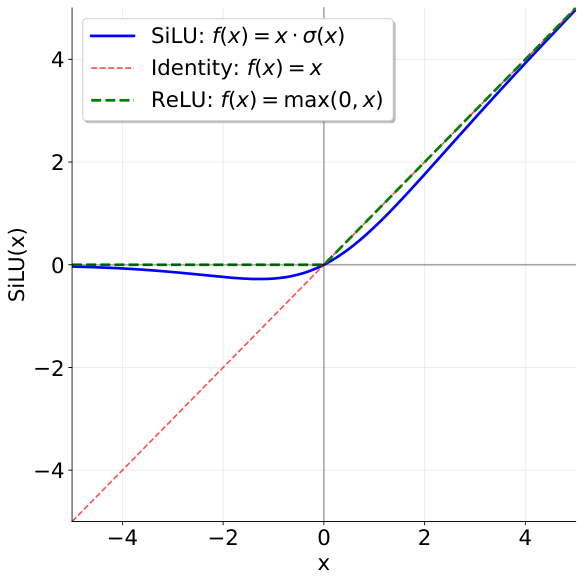
\includegraphics[width=0.6\textwidth]{figures/p21_v25.png}
\caption*{图 3：SiLU（又称 Swish）与 ReLU 激活函数的比较。}
\end{figure}

在最初的 Transformer 论文（A.~Vaswani et al.~[8] 的第 3.3 节）中，Transformer 前馈网络由两个线性变换组成，中间夹一个 ReLU 激活（$\operatorname{ReLU}(x) = \max(0, x)$）。在那个原始架构中，前馈内层的维度通常是输入维度的 4 倍。

然而，与这一原始设计相比，现代语言模型往往包含两点主要改动：使用另一种激活函数，并采用门控机制（gating mechanism）。具体来说，我们将实现 Llama 3（A.~Grattafiori et al., 2024）和 Qwen 2.5（A.~Yang et al., 2024）等大语言模型采用的 ``SwiGLU'' 激活函数，它把 SiLU（常称为 Swish）激活与一种叫做门控线性单元（Gated Linear Unit，GLU）的门控机制结合起来。我们还会仿照 PaLM（A.~Chowdhery et al., 2022）以来的大多数现代大语言模型（以及 LLaMA，H.~Touvron et al., 2023），省略线性层中有时使用的偏置项。

SiLU（即 Swish）激活函数（D.~Hendrycks et al., 2016；S.~Elfwing et al., 2017）定义如下：
\begin{equation}
\operatorname{SiLU}(x) = x \cdot \sigma(x) = \frac{x}{1 + e^{-x}}
\tag{5}
\end{equation}
如图~3 所示，SiLU 激活函数与 ReLU 激活函数相似，但在零点处是光滑的。

门控线性单元（GLU）最初由 Y.~N.~Dauphin et al.~[19] 定义为一个经过 sigmoid 函数的线性变换与另一个线性变换的逐元素乘积：
\begin{equation}
\operatorname{GLU}(x, W_1, W_2) = \sigma(W_1 x) \odot W_2 x,
\tag{6}
\end{equation}
其中 $\odot$ 表示逐元素乘法。据称门控线性单元能够``在保留非线性能力的同时，为梯度提供一条线性通路，从而缓解深层架构中的梯度消失问题''。

把 SiLU/Swish 与 GLU 结合起来，就得到 SwiGLU，我们将把它用于我们的前馈网络：
\begin{equation}
\operatorname{FFN}(x) = \operatorname{SwiGLU}(x, W_1, W_2, W_3) = W_2\bigl(\operatorname{SiLU}(W_1 x) \odot W_3 x\bigr),
\tag{7}
\end{equation}
其中 $x \in \mathbb{R}^{d_{\mathrm{model}}}$，$W_1, W_3 \in \mathbb{R}^{d_{\mathrm{ff}} \times d_{\mathrm{model}}}$，$W_2 \in \mathbb{R}^{d_{\mathrm{model}} \times d_{\mathrm{ff}}}$，且规范上取 $d_{\mathrm{ff}} = \tfrac{8}{3} d_{\mathrm{model}}$。在具体实现中，为了硬件效率，把这个数值取整到邻近的 64 的倍数即可。

N.~Shazeer~[20] 最先提出把 SiLU/Swish 激活与 GLU 结合，并通过实验表明，在语言建模任务上 SwiGLU 优于 ReLU 和 SiLU（无门控）等基线。在本作业的后面，你也会比较 SwiGLU 和 SiLU。虽然我们已经给出了一些关于这些组件的启发式论证（相关论文也提供了更多支持证据），但保持经验性的视角总是好的：Shazeer 论文中如今很有名的一句话是

\begin{quote}
``对于这些架构为何看似有效，我们不给出任何解释；与其他一切原因一样，我们把它们的成功归功于上天的仁慈（divine benevolence）。''
\end{quote}

\subsubsection*{问题（positionwise\_feedforward）：实现逐位置前馈网络（2 分）}

\textbf{交付要求：}实现由 SiLU 激活函数与 GLU 组成的 SwiGLU 前馈网络。

\textbf{注意：}在这个特定场景中，出于数值稳定性考虑，你可以放心地在实现中使用 \tm{torch.sigmoid}。

在实现中，你应把 $d_{\mathrm{ff}}$ 设为约 $\tfrac{8}{3} \times d_{\mathrm{model}}$，同时确保前馈内层的维度是 64 的倍数，以充分利用你的硬件。要对照我们提供的测试来检验你的实现，你需要在 \tm{[adapters.run\_swiglu]} 处实现测试适配器，然后运行 \tm{uv run pytest -k test\_swiglu} 来测试你的实现。

\subsubsection{相对位置嵌入（Relative Positional Embeddings）}

为了向模型注入位置信息，我们将实现旋转位置嵌入（Rotary Position Embeddings，常称 RoPE；J.~Su et al., 2021）。对于处于 token 位置 $i$ 的查询 token $q^{(i)} = W_q x^{(i)} \in \mathbb{R}^d$，我们将施加一个成对旋转矩阵 $R^i$，得到 $q'^{(i)} = R^i q^{(i)} = R^i W_q x^{(i)}$。这里，$R^i$ 会把嵌入元素对 $q^{(i)}_{2k-1:2k}$ 当作二维向量旋转角度
\[
\theta_{i,k} = \frac{i}{\Theta^{(2k-2)/d}}, \quad k \in \{1, \ldots, d/2\},
\]
其中 $\Theta$ 是某个常数。于是，我们可以把 $R^i$ 看作一个 $d \times d$ 的分块对角矩阵，其对角块为 $R^i_k$（$k \in \{1, \ldots, d/2\}$）：
\begin{equation}
R^i_k =
\begin{pmatrix}
\cos(\theta_{i,k}) & -\sin(\theta_{i,k}) \\
\sin(\theta_{i,k}) & \cos(\theta_{i,k})
\end{pmatrix}
\tag{8}
\end{equation}
这样我们就得到完整的旋转矩阵
\begin{equation}
R^i =
\begin{pmatrix}
R^i_1 & 0 & 0 & \cdots & 0 \\
0 & R^i_2 & 0 & \cdots & 0 \\
0 & 0 & R^i_3 & \cdots & 0 \\
\vdots & \vdots & \vdots & \ddots & \vdots \\
0 & 0 & 0 & \cdots & R^i_{d/2}
\end{pmatrix},
\tag{9}
\end{equation}
其中 0 表示 $2 \times 2$ 零矩阵。虽然可以直接构造出完整的 $d \times d$ 矩阵，但一个好的实现应当利用该矩阵的性质来更高效地完成变换。由于我们只关心给定序列内 token 之间的相对旋转，因此对 $\cos(\theta_{i,k})$ 和 $\sin(\theta_{i,k})$ 计算出的值可以在不同层、不同批次之间复用。如果你想进一步优化，可以只用一个 RoPE 模块供所有层引用，并在初始化时用 \tm{self.register\_buffer(persistent=False)} 预先创建一个 sin 与 cos 值的二维缓冲区（buffer），而不是 \tm{nn.Parameter}（因为我们不想学习这些固定的余弦和正弦值）。接下来，对我们作用于 $q^{(i)}$ 的完全相同的旋转过程，也要施加于 $k^{(j)}$，即用相应的 $R^j$ 做旋转。注意，这一层没有任何可学习参数。

\subsubsection*{问题（rope）：实现 RoPE（2 分）}

\textbf{交付要求：}实现一个对输入张量施加 RoPE 的 \tm{RotaryPositionalEmbedding} 类。

推荐使用如下接口：

\tm{def \_\_init\_\_(self, theta: float, d\_k: int, max\_seq\_len: int, device=None)}\quad 构造 RoPE 模块，并在需要时创建缓冲区。
\begin{itemize}
  \item \tm{theta: float}：RoPE 的 $\Theta$ 值。
  \item \tm{d\_k: int}：查询和键向量的维度。
  \item \tm{max\_seq\_len: int}：将输入的最大序列长度。
  \item \tm{device: torch.device | None = None}：缓冲区存储所在的设备。
\end{itemize}

\tm{def forward(self, x: torch.Tensor, token\_positions: torch.Tensor) -> torch.Tensor}\quad 处理形状为 \tm{(..., seq\_len, d\_k)} 的输入张量并返回相同形状的张量。注意，你应当容忍 $x$ 带有任意数量的批次维度。你应当假定 token 位置是形状为 \tm{(..., seq\_len)} 的张量，指定 $x$ 沿序列维度的 token 位置。

你应当使用 token 位置，沿序列维度对你（可能预先计算好的）cos 和 sin 张量做切片。

要测试你的实现，请完成 \tm{[adapters.run\_rope]}，并确保它能通过 \tm{uv run pytest -k test\_rope}。

\subsubsection{缩放点积注意力（Scaled Dot-Product Attention）}

接下来，我们将按照 A.~Vaswani et al.~[8]（第 3.2.1 节）的描述实现缩放点积注意力。作为预备步骤，Attention 运算的定义会用到 softmax——一种把未归一化的分数向量变成归一化分布的运算：
\begin{equation}
\operatorname{softmax}(v)_i = \frac{\exp(v_i)}{\sum_{j=1}^{n} \exp(v_j)}.
\tag{10}
\end{equation}

注意，当数值较大时 $\exp(v_i)$ 可能变为 inf（此时 $\tfrac{\inf}{\inf} = $ NaN）。注意到 softmax 运算对``给所有输入加上同一常数 $c$''保持不变，就可以避免这个问题。我们可以利用这一性质来保证数值稳定性——通常做法是把 $v$ 的最大元素从 $v$ 的所有元素中减去，使新的最大元素为 0。接下来你就要实现 softmax，并使用这一技巧来保证数值稳定性。

\subsubsection*{问题（softmax）：实现 softmax（1 分）}

\textbf{交付要求：}编写一个对张量施加 softmax 运算的函数。该函数应接受两个参数：一个张量和一个\textit{维度} $i$，并对输入张量的第 $i$ 个维度施加 softmax。输出张量应与输入张量形状相同，但其第 $i$ 个维度上应是一个归一化的概率分布。请使用``从第 $i$ 个维度的所有元素中减去该维度最大值''的技巧，以避免数值稳定性问题。

{\sloppy
要测试你的实现，请完成 \tm{[adapters.run\_softmax]}，并确保它能通过 \tm{uv run pytest -k test\_softmax\_matches\_pytorch}。
\par}

现在我们可以从数学上定义 Attention 运算：
\begin{equation}
\operatorname{Attention}(Q, K, V) = \operatorname{softmax}\!\left(\frac{QK^{\top}}{\sqrt{d_k}}\right)V
\tag{11}
\end{equation}
其中 $Q \in \mathbb{R}^{n \times d_k}$，$K \in \mathbb{R}^{m \times d_k}$，$V \in \mathbb{R}^{m \times d_v}$。这里 $Q$、$K$、$V$ 都是该运算的输入——注意它们不是可学习参数。

\textbf{掩码（Masking）：}有时，对 attention 运算的输出做\textit{掩码}（mask）会很方便。掩码应具有 $M \in \{\text{True}, \text{False}\}^{n \times m}$ 的形状，这个布尔矩阵的第 $i$ 行指示查询 $i$ 应该关注（attend to）哪些键。按照惯例（这有点容易让人混淆），位置 $(i, j)$ 上的 \tm{True} 表示查询 $i$ \textit{确实}关注键 $j$，而 \tm{False} 表示查询\textit{不}关注该键。换句话说，``信息流动''发生在值为 \tm{True} 的 $(i, j)$ 位置上。例如，考虑一个元素为 \tm{[[True, True, False]]} 的 $1 \times 3$ 掩码矩阵：这个唯一的查询向量只关注前两个键。

从计算角度看，使用掩码比对子序列分别计算 attention 高效得多；具体做法是取 softmax 之前的值（$QK^{\top} / \sqrt{d_k}$），并在掩码矩阵为 \tm{False} 的任何位置加上 $-\infty$。

\subsubsection*{问题（scaled\_dot\_product\_attention）：实现缩放点积注意力（5 分）}

\textbf{交付要求：}实现缩放点积注意力函数。你的实现应当处理形状为 \tm{(batch\_size, ..., seq\_len, d\_k)} 的键和查询，以及形状为 \tm{(batch\_size, ..., seq\_len, d\_v)} 的值，其中 \tm{...} 表示任意数量（如果提供的话）的其他类批次（batch-like）维度。实现应返回形状为 \tm{(batch\_size, ..., seq\_len, d\_v)} 的输出。关于类批次维度的讨论见第 3.2 节。

你的实现还应支持一个可选的、由使用者提供的形状为 \tm{(seq\_len, seq\_len)} 的布尔掩码。掩码值为 \tm{True} 的位置，其注意力概率合计应为 1；掩码值为 \tm{False} 的位置，其注意力概率应为 0。

要对照我们提供的测试来检验你的实现，你需要在 \tm{[adapters.run\_scaled\_dot\_product\_attention]} 处实现测试适配器。\tm{uv run pytest -k test\_scaled\_dot\_product\_attention} 在三阶输入张量上测试你的实现，而 \tm{uv run pytest -k test\_4d\_scaled\_dot\_product\_attention} 在四阶输入张量上测试你的实现。

\subsubsection{因果多头自注意力（Causal Multi-Head Self-Attention）}

我们将按照 A.~Vaswani et al.~[8] 第 3.2.2 节的描述实现多头自注意力。回顾一下，从数学上讲，多头注意力的运算定义如下：
\begin{equation}
\operatorname{MultiHead}(Q, K, V) = \operatorname{Concat}(\text{head}_1, \ldots, \text{head}_h)
\tag{12}
\end{equation}
\begin{equation}
\text{其中 } \text{head}_i = \operatorname{Attention}(Q_i, K_i, V_i)
\tag{13}
\end{equation}
其中 $Q_i$、$K_i$、$V_i$ 分别是 $Q$、$K$、$V$ 的嵌入维度中编号为 $i \in \{1, \ldots, h\}$、大小为 $d_k$ 或 $d_v$ 的切片。这里的 \tm{Attention} 就是第 3.4.4 节定义的缩放点积注意力运算。由此我们可以构造多头自注意力运算：
\begin{equation}
\operatorname{MultiHeadSelfAttention}(x) = W_O \operatorname{MultiHead}(W_Q x, W_K x, W_V x)
\tag{14}
\end{equation}
这里，可学习参数是 $W_Q \in \mathbb{R}^{d_k \times d_{\mathrm{model}}}$、$W_K \in \mathbb{R}^{d_k \times d_{\mathrm{model}}}$、$W_V \in \mathbb{R}^{d_v \times d_{\mathrm{model}}}$，以及 $W_O \in \mathbb{R}^{d_{\mathrm{model}} \times d_h}$。由于 $Q$、$K$、$V$ 在多头注意力运算中被切片，我们可以把 $W_Q$、$W_K$、$W_V$ 看作沿输出维度为每个头分开。当你把这一切跑通时，key、value 和 query 三个投影总共应当只做三次矩阵乘法。\footnote{作为更高的挑战目标（stretch goal），可以尝试把 key、query、value 三个投影合并成一个权重矩阵，这样你只需要一次矩阵乘法。}

\textbf{因果掩码（Causal masking）}

你的实现应当阻止模型关注序列中未来的 token。换言之，如果模型得到 token 序列 $t_1, \ldots, t_n$，而我们要计算前缀 $t_1, \ldots, t_i$（其中 $i < n$）的下一个词预测，那么模型应当\textit{不能}访问（关注）位置 $t_{i+1}, \ldots, t_n$ 处的 token 表示，因为在推理阶段生成文本时它本来就拿不到这些 token（而且这些未来的 token 会泄露关于真实下一个词的身份信息，使语言建模预训练目标变得平凡）。对于输入 token 序列 $t_1, \ldots, t_n$，一种朴素的做法是把多头自注意力运行 $n$ 次（对应序列中 $n$ 个不同的前缀），以阻止对未来 token 的访问。但我们将改用因果注意力掩码（causal attention masking），它允许 token $i$ 关注序列中所有满足 $j \le i$ 的位置 $j$。你可以使用 \tm{torch.triu} 或广播的索引比较来构造这个掩码，并且应当利用第 3.4.4 节的缩放点积注意力实现已支持注意力掩码这一事实。

\textbf{应用 RoPE（Applying RoPE）}

RoPE 应施加在查询和键向量上，而不是值向量。另外，头（head）维度应当作为批次维度处理，因为在多头注意力中，注意力是对每个头独立施加的。这意味着对每个头的查询和键向量，施加的 RoPE 旋转应当完全相同。

\subsubsection*{问题（multihead\_self\_attention）：实现因果多头自注意力（5 分）}

\textbf{交付要求：}把因果多头自注意力实现为一个 \tm{torch.nn.Module}。你的实现应当（至少）接受以下参数：
\begin{itemize}
  \item \tm{d\_model: int}：Transformer 块输入的维度。
  \item \tm{num\_heads: int}：多头自注意力中使用的头数。
\end{itemize}
按照 A.~Vaswani et al.~[8]，设 $d_k = d_v = \tfrac{d_{\mathrm{model}}}{h}$。要对照我们提供的测试来检验你的实现，请在 \tm{[adapters.run\_multihead\_self\_attention]} 处实现测试适配器，然后运行 \tm{uv run pytest -k \allowbreak test\_multihead\_self\_attention} 来测试你的实现。

\subsection{完整的 Transformer 语言模型}

我们先从组装 Transformer 块开始（回顾图~2 会很有帮助）。Transformer 块包含两个``子层''：一个用于多头自注意力，另一个用于 SwiGLU 前馈网络。在每个子层中，我们先执行 RMSNorm，然后执行主运算（MHA/FF），最后加上残差连接。

具体来说，Transformer 块的前半部分（第一个``子层''）应实现下面这组更新，从输入 $x$ 产生输出 $y$：
\begin{equation}
y = x + \operatorname{MultiHeadSelfAttention}(\operatorname{RMSNorm}(x)).
\tag{15}
\end{equation}

\subsubsection*{问题（transformer\_block）：实现 Transformer 块（3 分）}

按照第 3.4 节的描述和图~2 的示意，实现 pre-norm Transformer 块。你的 Transformer 块应当（至少）接受以下参数：
\begin{itemize}
  \item \tm{d\_model: int}：Transformer 块输入的维度。
  \item \tm{num\_heads: int}：多头自注意力中使用的头数。
  \item \tm{d\_ff: int}：逐位置前馈内层的维度。
\end{itemize}
要测试你的实现，请实现适配器 \tm{[adapters.run\_transformer\_block]}，然后运行 \tm{uv run pytest -k test\_transformer\_block} 来测试你的实现。

\textbf{交付要求：}能通过所提供测试的 Transformer 块代码。

现在我们按照图~1 的高层示意图把各个块拼装起来。按照第 3.1.0.1 节对嵌入的描述完成嵌入，把它输入 \tm{num\_layers} 个 Transformer 块，然后再送入最后的层归一化和 LM head，得到词表上的未归一化分布（即 logits）。

\subsubsection*{问题（transformer\_lm）：实现 Transformer 语言模型（3 分）}

是时候把它们全部组合起来了！请按照第 3.1 节的描述和图~1 的示意实现 Transformer 语言模型。至少，你的实现应当接受 Transformer 块的所有上述构造参数，以及下面这些额外参数：
\begin{itemize}
  \item \tm{vocab\_size: int}：词表大小，用于确定 token 嵌入矩阵的维度。
  \item \tm{context\_length: int}：最大上下文长度，用于确定 RoPE 的 sin 和 cos 缓冲区的维度。
  \item \tm{num\_layers: int}：使用的 Transformer 块数量。
\end{itemize}
要对照我们提供的测试来检验你的实现，你首先需要在 \tm{[adapters.run\_transformer\_lm]} 处实现测试适配器，然后运行 \tm{uv run pytest -k test\_transformer\_lm} 来测试你的实现。

\textbf{交付要求：}能通过上述测试的 Transformer 语言模型模块。

\textbf{资源核算（Resource accounting）}

了解 Transformer 各个部分如何消耗计算和内存是很有用的。我们将逐步完成一些基本的 ``FLOPs 核算''。Transformer 中的 FLOPs 的\textit{绝大部分}是矩阵乘法，所以我们的核心方法很简单：
\begin{enumerate}
  \item 写出 Transformer 前向传播中的所有矩阵乘法。
  \item 把每个矩阵乘法换算成所需的 FLOPs。
\end{enumerate}
对于第二步，下面的事实会很有用：

\begin{quote}
\textbf{法则：}给定 $A \in \mathbb{R}^{m \times n}$ 和 $B \in \mathbb{R}^{n \times p}$，矩阵--矩阵乘积 $AB$ 需要 $2mnp$ 个 FLOPs。
\end{quote}

为什么？注意 $(AB)[i, j] = A[i, :] \cdot B[:, j]$，而这个点积需要 $n$ 次加法和 $n$ 次乘法（$2n$ 个 FLOPs）。又因为矩阵--矩阵乘积 $AB$ 有 $m \times p$ 个元素，所以 FLOPs 总数为 $(2n)(mp) = 2mnp$。

在做下一道题之前，建议先把你的 Transformer 块和 Transformer 语言模型的每个组件过一遍，列出所有矩阵乘法及其对应的 FLOPs 开销。

\subsubsection*{问题（transformer\_accounting）：Transformer 语言模型资源核算（5 分）}

\begin{enumerate}
  \item[(a)] 考虑一个使用本作业架构的 GPT-2 XL 规模模型，它具有如下配置：
  \begin{itemize}
    \item \tm{vocab\_size}: 50,257
    \item \tm{context\_length}: 1,024
    \item \tm{num\_layers}: 48
    \item \tm{d\_model}: 1,600
    \item \tm{num\_heads}: 25
    \item \tm{d\_ff}: 4,288（$\tfrac{8}{3} \times 1{,}600$ 最接近的 64 的倍数）
  \end{itemize}

  假设我们用这个配置构建模型。我们的模型会有多少个可训练参数？假设每个参数用单精度浮点数表示，仅加载这个模型需要多少内存？

  \textbf{交付要求：}一到两句话的回答。

  \item[(b)] 找出完成一次 GPT-2 XL 形状模型前向传播所需的矩阵乘法。这些矩阵乘法总共需要多少 FLOPs？假设输入序列有 \tm{context\_length} 个 token。

  \textbf{交付要求：}一份矩阵乘法列表（附说明）以及所需 FLOPs 的总数。

  \item[(c)] 根据你上面的分析，模型的哪些部分需要最多的 FLOPs？

  \textbf{交付要求：}一到两句话的回答。

  \item[(d)] 对 GPT-2 small（12 层，768 \tm{d\_model}，12 头）、GPT-2 medium（24 层，1024 \tm{d\_model}，16 头）和 GPT-2 large（36 层，1280 \tm{d\_model}，20 头）重复你的分析。随着模型规模增大，Transformer 语言模型的哪些部分占总 FLOPs 的比例变大了，哪些变小了？

  \textbf{交付要求：}对每个模型，给出模型组件及其对应 FLOPs 的分解（占前向传播所需总 FLOPs 的比例）。此外，用一到两句话描述模型规模的变化如何改变各组件 FLOPs 的占比。

  \item[(e)] 取 GPT-2 XL 并把上下文长度增加到 16,384。一次前向传播的总 FLOPs 会如何变化？各模型组件 FLOPs 的相对占比会如何变化？

  \textbf{交付要求：}一到两句话的回答。
\end{enumerate}

\section{训练 Transformer 语言模型}

现在我们已有预处理数据（通过分词器）和模型（Transformer）的步骤，剩下的是构建支持训练的全部代码。这包括以下几部分：
\begin{itemize}
  \item \textbf{损失（Loss）}：我们需要定义损失函数（交叉熵）。
  \item \textbf{优化器（Optimizer）}：我们需要定义最小化该损失的优化器（AdamW）。
  \item \textbf{训练循环（Training loop）}：我们需要所有配套的基础设施，用于加载数据、保存检查点（checkpoint）并管理训练。
\end{itemize}

\subsection{交叉熵损失（Cross-entropy loss）}

回顾一下，Transformer 语言模型为每条长度为 $m + 1$ 的序列 $x$ 和每个 $i = 1, \ldots, m$ 定义分布 $p_\theta(x_{i+1} \mid x_{1:i})$。给定一个由长度为 $m + 1$ 的序列组成的训练集 $D$，我们定义标准的交叉熵（负对数似然）损失函数：
\begin{equation}
\ell(\theta; D) = \frac{1}{|D|\, m} \sum_{x \in D} \sum_{i=1}^{m} -\log p_\theta(x_{i+1} \mid x_{1:i}).
\tag{16}
\end{equation}
（注意，Transformer 的一次前向传播就能同时得到所有 $i = 1, \ldots, m$ 的 $p_\theta(x_{i+1} \mid x_{1:i})$。）

具体来说，Transformer 会为每个位置 $i$ 计算 logits $o_i \in \mathbb{R}^{\text{vocab size}}$，由此得到：\footnote{注意 $o_i[k]$ 指向量 $o_i$ 中下标为 $k$ 的值。}
\begin{equation}
p(x_{i+1} \mid x_{1:i}) = \operatorname{softmax}(o_i)[x_{i+1}] = \frac{\exp\bigl(o_i[x_{i+1}]\bigr)}{\sum_{a=1}^{\text{vocab size}} \exp(o_i[a])}.
\tag{17}
\end{equation}
交叉熵损失通常是相对于 logits 向量 $o_i \in \mathbb{R}^{\text{vocab size}}$ 和目标 $x_{i+1}$ 定义的。\footnote{这对应于 $x_{i+1}$ 上的 Dirac delta 分布与预测分布 $\operatorname{softmax}(o_i)$ 之间的交叉熵。}

实现交叉熵损失时需要像 softmax 一样小心处理数值问题。

\subsubsection*{问题（cross\_entropy）：实现交叉熵（1 分）}

\textbf{交付要求：}编写一个计算交叉熵损失的函数，它接收预测的 logits（$o_i$）和目标（$x_{i+1}$），并计算交叉熵 $\ell_i = -\log \operatorname{softmax}(o_i)[x_{i+1}]$。你的函数应做到以下几点：
\begin{itemize}
  \item 为数值稳定性减去最大元素。
  \item 尽可能地约去 log 和 exp。
  \item 处理任意额外的批次维度，并返回整个批次的\textit{平均}值。与第 3.2 节一样，我们假定类批次维度总是排在词表大小维度之前。
\end{itemize}
请实现 \tm{[adapters.run\_cross\_entropy]}，然后运行 \tm{uv run pytest -k test\_cross\_entropy} 来测试你的实现。

\textbf{困惑度（Perplexity）}

交叉熵用于训练已经足够，但在评估模型时，我们还想报告困惑度（perplexity）。对于长度为 $m$、交叉熵损失依次为 $\ell_1, \ldots, \ell_m$ 的序列：
\begin{equation}
\text{perplexity} = \exp\!\left(\frac{1}{m} \sum_{i=1}^{m} \ell_i\right).
\tag{18}
\end{equation}

\subsection{SGD 优化器}

有了损失函数之后，我们开始探索优化器。最简单的基于梯度的优化器是随机梯度下降（Stochastic Gradient Descent，SGD）。我们从随机初始化的参数 $\theta_0$ 出发，然后在每一步 $t = 0, \ldots, T-1$ 执行如下更新：
\begin{equation}
\theta_{t+1} \leftarrow \theta_t - \alpha_t \nabla L(\theta_t; B_t),
\tag{19}
\end{equation}
其中 $B_t$ 是从数据集 $D$ 中随机采样的一个批次（batch）数据，而\textit{学习率}（learning rate）$\alpha_t$ 和\textit{批次大小}（batch size）$|B_t|$ 是超参数。

\subsubsection{在 PyTorch 中实现 SGD（Implementing SGD in PyTorch）}

要实现我们的优化器，我们将继承 PyTorch 的 \tm{torch.optim.Optimizer} 类。\tm{Optimizer} 子类必须实现两个方法：

\tm{def \_\_init\_\_(self, params, ...)}\quad 应完成优化器的初始化。这里 \tm{params} 是待优化参数的集合（或参数组，以便用户可以对模型的不同部分使用不同的超参数，例如不同的学习率）。务必把 \tm{params} 传给基类的 \tm{\_\_init\_\_} 方法，基类会存储这些参数供 \tm{step} 使用。你可以根据优化器需要接受额外的参数（例如学习率就是一个常见的参数），并把它们以字典的形式传给基类构造函数，字典的键就是你自己为这些参数起的名称（字符串）。

\tm{def step(self)}\quad 应对参数做一次更新。在训练循环中，它会在反向传播之后被调用，因此你可以拿到上一个批次的梯度。该方法应遍历每个参数张量 \tm{p} 并\textit{就地}（in place）修改它们，也就是设置 \tm{p.data}——它是与该参数相关联的张量——依据梯度 \tm{p.grad}（如果存在），即损失关于该参数的梯度张量。

PyTorch 的优化器 API 有一些微妙之处，所以用一个例子来讲解会更容易。为了让例子更丰富，我们实现 SGD 的一个小变体：学习率随训练衰减，从初始学习率 $\alpha$ 开始，随时间采取越来越小的步长：
\begin{equation}
\theta_{t+1} = \theta_t - \frac{\alpha}{\sqrt{t+1}} \nabla L(\theta_t; B_t)
\tag{20}
\end{equation}
我们来看看这个版本的 SGD 如何实现为一个 PyTorch \tm{Optimizer}：

\begin{lstlisting}
from collections.abc import Callable, Iterable
from typing import Optional
import torch
import math

class SGD(torch.optim.Optimizer):
    def __init__(self, params, lr=1e-3):
        if lr < 0:
            raise ValueError(f"Invalid learning rate: {lr}")
        defaults = {"lr": lr}
        super().__init__(params, defaults)

    def step(self, closure: Optional[Callable] = None):
        loss = None if closure is None else closure()
        for group in self.param_groups:
            lr = group["lr"]  # 获取学习率。
            for p in group["params"]:
                if p.grad is None:
                    continue

                state = self.state[p]  # 获取与 p 相关联的状态。
                t = state.get("t", 0)  # 从状态中取出迭代次数，若无则为 0。
                grad = p.grad.data  # 获取损失关于 p 的梯度。
                p.data -= lr / math.sqrt(t + 1) * grad  # 就地更新权重张量。
                state["t"] = t + 1  # 迭代次数加一。

        return loss
\end{lstlisting}

在 \tm{\_\_init\_\_} 中，我们把参数以及默认超参数传给基类构造函数（参数可能是分组传入的，每组有各自不同的超参数）。如果参数只是单个 \tm{torch.nn.Parameter} 对象的集合，基类构造函数会创建一个单独的组，并为其指定默认超参数。然后，在 \tm{step} 中，我们遍历每个参数组，再遍历该组中的每个参数，并应用式~(20)。这里，我们把迭代次数作为与每个参数相关联的状态来保存：先读取这个值，在梯度更新中使用它，然后再更新它。该 API 规定，用户可以传入一个可调用对象 \tm{closure}，在优化器步进之前重新计算损失。对我们将要使用的优化器来说用不到它，但为了符合 API 我们还是加上了。

为了看看它如何工作，我们可以用下面这个\textit{训练循环}（training loop）的最小示例：

\begin{lstlisting}
weights = torch.nn.Parameter(5 * torch.randn((10, 10)))
opt = SGD([weights], lr=1)

for t in range(100):
    opt.zero_grad()  # 重置所有可学习参数的梯度。
    loss = (weights**2).mean()  # 计算一个标量损失值。
    print(loss.cpu().item())
    loss.backward()  # 运行反向传播，计算梯度。
    opt.step()  # 运行优化器步进。
\end{lstlisting}

这就是训练循环的典型结构：在每次迭代中，我们计算损失并执行一步优化器。训练语言模型时，我们的可学习参数来自模型（在 PyTorch 中，\tm{m.parameters()} 会给出这个集合）。损失将在采样出的一个数据批次上计算，但训练循环的基本结构不变。

\subsubsection*{问题（learning\_rate\_tuning）：调整学习率（1 分）}

正如我们将看到的，对训练影响最大的超参数之一就是学习率。让我们在上面的玩具示例中实际感受一下。把上面的 SGD 示例分别用另外三个学习率 \tm{1e1}、\tm{1e2} 和 \tm{1e3} 运行，只训练 10 次迭代。每个学习率下损失会发生什么？它衰减得更快、更慢，还是会发散（即随训练进行不断增大）？

\textbf{交付要求：}用一到两句话描述你观察到的行为。

\subsection{AdamW}

现代语言模型通常不再用 SGD，而是用更复杂的优化器来训练。近来使用的优化器大多源自 Adam 优化器（D.~P.~Kingma et al., 2015）。我们将使用 AdamW（I.~Loshchilov et al., 2019），它在近期工作中被广泛使用。AdamW 对 Adam 提出了一处改进：通过加入\textit{权重衰减}（weight decay，每次迭代把参数向 0 拉近）来改善正则化，而且这种衰减与梯度更新是解耦的。我们将按照 I.~Loshchilov et al.~[23] 的算法 2 来实现 AdamW。

AdamW 是\textit{有状态的}（stateful）：它为每个参数维护其第一矩和第二矩的滚动估计。因此，AdamW 用额外的内存换取更好的稳定性和收敛性。除了学习率 $\alpha$ 之外，AdamW 还有一对控制矩估计更新的超参数 $(\beta_1, \beta_2)$，以及一个权重衰减率 $\lambda$。一般应用把 $(\beta_1, \beta_2)$ 设为 $(0.9, 0.999)$，但 LLaMA（H.~Touvron et al., 2023）和 GPT-3（T.~B.~Brown et al., 2020）这类大语言模型常用 $(0.9, 0.95)$ 来训练。该算法可以写作如下形式，其中 $\varepsilon$ 是一个很小的值（例如 $10^{-8}$），用于在 $v$ 中出现极小值时改善数值稳定性：

\begin{table}[htbp]
\centering
\begin{tabular}{@{}ll@{}}
\toprule
\multicolumn{2}{@{}l@{}}{\textbf{算法 1}：AdamW 优化器} \\
\midrule
1 & $\text{init}(\theta)$ \quad $\triangleright$ 初始化可学习参数 \\
2 & $m \leftarrow 0$ \quad $\triangleright$ 第一矩向量的初始值；与 $\theta$ 形状相同 \\
3 & $v \leftarrow 0$ \quad $\triangleright$ 第二矩向量的初始值；与 $\theta$ 形状相同 \\
4 & \textbf{for} $t = 1, \ldots, T$ \textbf{do} \\
5 & \quad 采样一个数据批次 $B_t$ \\
6 & \quad $g \leftarrow \nabla_\theta \ell(\theta; B_t)$ \quad $\triangleright$ 计算损失的梯度 \\
7 & \quad $\alpha_t \leftarrow \alpha\, \frac{\sqrt{1-\beta_2^t}}{1-\beta_1^t}$ \quad $\triangleright$ 为第 $t$ 次迭代计算调整后的 $\alpha$ \\
8 & \quad $\theta \leftarrow \theta - \alpha \lambda \theta$ \quad $\triangleright$ 施加权重衰减 \\
9 & \quad $m \leftarrow \beta_1 m + (1 - \beta_1) g$ \quad $\triangleright$ 更新第一矩估计 \\
10 & \quad $v \leftarrow \beta_2 v + (1 - \beta_2) g^2$ \quad $\triangleright$ 更新第二矩估计 \\
11 & \quad $\theta \leftarrow \theta - \alpha_t \frac{m}{\sqrt{v} + \varepsilon}$ \quad $\triangleright$ 施加经矩调整的权重更新 \\
12 & \textbf{end for} \\
\bottomrule
\end{tabular}
\caption*{算法 1：AdamW 优化器伪代码。}
\end{table}

注意 $t$ 从 1 开始。接下来你就要实现这个优化器。

\subsubsection*{问题（adamw）：实现 AdamW（2 分）}

\textbf{交付要求：}把 AdamW 优化器实现为 \tm{torch.optim.Optimizer} 的子类。你的类应在 \tm{\_\_init\_\_} 中接收学习率 $\alpha$，以及 $\beta$、$\varepsilon$ 和 $\lambda$ 超参数。为了帮你保存状态，基类 \tm{Optimizer} 为你提供了一个字典 \tm{self.state}，它把 \tm{nn.Parameter} 对象映射到一个字典，用于存储该参数所需的任何信息（对 AdamW 而言就是矩估计）。请实现 \tm{[adapters.get\_adamw\_cls]}，并确保它能通过 \tm{uv run pytest -k test\_adamw}。

\subsubsection*{问题（adamw\_accounting）：AdamW 训练的资源核算（2 分）}

我们来计算运行 AdamW 需要多少内存和计算。假设所有张量都使用 \tm{float32}。

\begin{enumerate}
  \item[(a)] 运行 AdamW 需要多少峰值内存？请把答案按参数、激活值、梯度和优化器状态的内存占用分解表示。答案请用 \tm{batch\_size} 和模型超参数（\tm{vocab\_size}、\tm{context\_length}、\tm{num\_layers}、\tm{d\_model}、\tm{num\_heads}）表示。假定 $d_{\mathrm{ff}} = \tfrac{8}{3} \times d_{\mathrm{model}}$。

  为简单起见，计算激活值的内存占用时只考虑以下组件：
  \begin{itemize}
    \item Transformer 块
    \begin{itemize}
      \item RMSNorm（各处）
      \item 多头自注意力子层：$QKV$ 投影、$QK^{\top}$ 矩阵乘法、softmax、对值的加权和、输出投影。
      \item 逐位置前馈（SwiGLU）：$W_1$、$W_2$、门控分支上的 SiLU、逐元素乘积、$W_3$
    \end{itemize}
  \end{itemize}
\end{enumerate}
